% AER-Article.tex for AEA last revised 22 June 2011
\documentclass[]{AEA}

% The mathtime package uses a Times font instead of Computer Modern.
% Uncomment the line below if you wish to use the mathtime package:
%\usepackage[cmbold]{mathtime}
% Note that miktex, by default, configures the mathtime package to use commercial fonts
% which you may not have. If you would like to use mathtime but you are seeing error
% messages about missing fonts (mtex.pfb, mtsy.pfb, or rmtmi.pfb) then please see
% the technical support document at http://www.aeaweb.org/templates/technical_support.pdf
% for instructions on fixing this problem.

% Note: you may use either harvard or natbib (but not both) to provide a wider
% variety of citation commands than latex supports natively. See below.

% Uncomment the next line to use the natbib package with bibtex
\usepackage{natbib}

% Uncomment the next line to use the harvard package with bibtex
%\usepackage[abbr]{harvard}

% This command determines the leading (vertical space between lines) in draft mode
% with 1.5 corresponding to "double" spacing.
\draftSpacing{1.5}

% For Pandoc highlighting needs

% Pandoc citation processing

\usepackage{graphicx}
\usepackage{amsmath}
\usepackage{amssymb}
\usepackage{placeins}
\usepackage{booktabs}
\usepackage{longtable}
\usepackage{array}
\usepackage{multirow}
\usepackage{wrapfig}
\usepackage{float}
\usepackage{colortbl}
\usepackage{pdflscape}
\usepackage{tabu}
\usepackage{threeparttable}
\usepackage{threeparttablex}
\usepackage[normalem]{ulem}
\usepackage{makecell}
\usepackage{xcolor}

\usepackage{hyperref}

\begin{document}

\title{Brother, Can You Spare a Manufacturing Job? How Voters React to
Deindustrialization}
\shortTitle{Brother, Can You Spare a Manufacturing Job?}
% \author{Author1 and Author2\thanks{Surname1: affiliation1, address1, email1.
% Surname2: affiliation2, address2, email2. Acknowledgements}}


\author{
  Catherine Darin\\
  Zagreb Mukerjee\thanks{
  Darin: Harvard University, \href{mailto:cdarin@hks.harvard.edu}{cdarin@hks.harvard.edu}.
  Mukerjee: Harvard University, \href{mailto:zagrebmukerjee@fas.harvard.edu}{zagrebmukerjee@fas.harvard.edu}.
  Code available at https://github.com/zagrebmukerjee/ReplicationPaper
}
}

\date{\today}
\pubMonth{12}
\pubYear{2021}
\pubVolume{}
\pubIssue{}
\JEL{}
\Keywords{}

\begin{abstract}
What led to Donald Trump's surprising 2016 election victory? This paper
examines the potential contribution of deindustrialization. We exploit
county-level differences in manufacturing density as a source of
exogenous variation, using both instrumental-variable regression and
covariate balancing methods. Counterintuitively, we find that counties
that gained manufacturing jobs from 2012-2015 are more likely to have
swung towards Trump. We believe this is due to an omitted variable - the
job loss experienced from 2004 to 2012. Counties that experienced prior
deindustrialization were more likely to exhibit increased support for
Trump, as well as a slight manufacturing rebound in 2012-2015.
Disaggregating this result by race shows that the Democratic vote share
fell where layoffs affected white populations, and rose where layoffs
affected nonwhites. This suggests a racial component to how voters
process economic hardship.
\end{abstract}


\maketitle

\section{Introduction} 
\label{Introduction}

This paper analyzes the relationship between deindustrialization, race,
and the election of Donald Trump in 2016. Previous analyses have focused
on the effects of racial animus, trade, or the conjunction of the two on
political polarization and election outcomes (\cite{Autor20};
\cite{Che16}; \cite{BR21}). We extend the analysis of \cite{Baccini21},
one of the first papers to examine the political effects of
deindustrialization while considering race and localization.

Deindustrialization - the transition of the U.S. economy away from
manufacturing - has led to widespread job loss and created adverse
knock-on effects for a wide swath of Americans. Our measure of
dindustrialization incorporates job losses due to trade with China and
others (see \cite{Acemoglu16}); it also includes job losses due to
automation, demand changes, and other factors. The experience of
deindustrialization has not been uniform; rather, it has been
concentrated in areas of the country that were previously economically
reliant on manufacturing. As shown in Figure \ref{ManuMap}, states
across the eastern half of America, particularly in the South and
Midwest, have experienced the most pronouncd manufacturing employment
losses. The localized nature of this analysis highlights the uneven and
concentrated harms of deindustrialization.

This paper analyzes the relationship between deindustrialization, race,
and the election of Donald Trump in 2016. Previous analysis has focused
on racial animus, trade, or the conjunction of the two on political
polarization and election outcomes (\cite{Autor20}; \cite{Che16};
\cite{BR21}). We extend the analysis of \cite{Baccini21}, one of the
first papers to examine the political effects of deindustrialization
that while considering race and localization. Deindustrialization - the
transition of the U.S. economy away from manufacturing - has led to
widespread job loss and created adverse knock-on effects for a wide
swath of Americans. Our measure of dindustrialization incorporates job
losses due to trade with China and others (see \cite{Acemoglu16}); it
also includes job losses due to automation, demand changes, and other
factors. The experience of deindustrialization has not been uniform;
rather, it has been concentrated in certain areas of the country that
were previously economically reliant on manufacturing, as demonstrated
in Figure \ref{ManuMap}. The localized nature of this analysis
highlights the uneven and concentrated harms of deindustrialization.

\FloatBarrier
\begin{figure} \label{ManuMap}
\caption{Concentration of Deindustrialization (2004-2015) in the eastern United States }

\begin{center}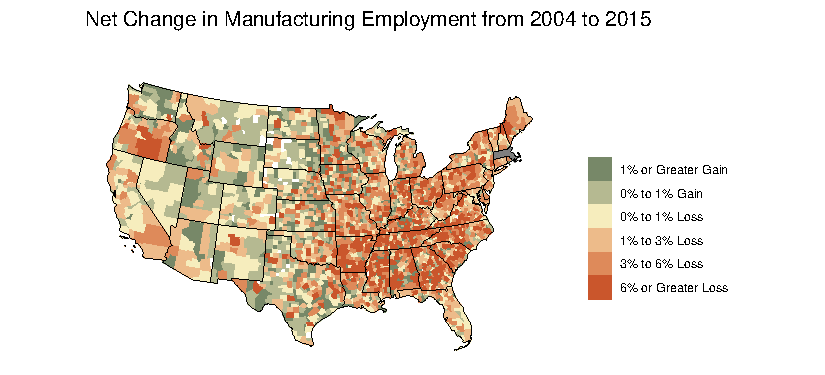
\includegraphics{Final-Draft_files/figure-latex/unnamed-chunk-2-1} \end{center}



\FloatBarrier
\begin{figurenotes}
Calculated at the county-level as the net change in manufacturing employment between 2004 and 2015 divided by 2004 total employment.
\end{figurenotes}
\end{figure}
\FloatBarrier

In their central analysis, \cite{Baccini21} analyzed the effect of gross
manufacturing job losses from 2012 to 2015 on the change in Democratic
vote share in the 2016 presidential election. \cite{Baccini21} find
evidence that the experience of deindustralization was associated with
support for Donald Trump, particularly among whites.

Our analysis extends \cite{Baccini21} in several ways. First, we change
focus from a measure of \emph{gross} losses in manufacturing jobs to
\emph{net} losses. As discussed in \ref{datasec}, we believe this to be
a more accurate measure of deindustrialization. Second, we change the
temporal focus. Rather than focusing on manufacturing job loss in
2012-2015, we extend our analysis back to 2004. This is an important
change. As shown in Figure \ref{natlPlotTS}, the bulk of U.S.
manufacturing job loss took place prior to 2012; in fact, the 2012-2015
period was characterized by a slight rebound in manufacturing jobs.
Finally, we augment the instrumental-variable approach with one based on
covariate balancing.

Like \cite{Baccini21}, we find evidence that the experience of
deindustralization was associated with support for Donald Trump,
particularly among whites. \cite{Baccini21} find that gross
manufacturing layoffs between 2012-2015 were associated with a loss in
Democratic vote share. However, using a different measure of
deindustrialization - \emph{net} change in manufacturing employment - we
find the oppposite effect: that counties with manufacturing job
\emph{gains} from 2012-2015 tended to swing towards Donald Trump in
2016. We extend the analysis to the 2004-2015 period in order to capture
the long-term effects of deindustrialization on a region. Doing so, we
find that regions experiencing more manufacturing job losses swung
towards Donald Trump in 2016, and that this occurred more when those
losing jobs were white.

Like \cite{Baccini21}, our results suggest that the experience of
deindustralization was associated with support for Donald Trump,
particularly among whites. However, our results differ from
\cite{Baccini21} in regards to the \emph{timing} of the impact of
manufacturing job losses on employment. In fact, using our preferred
measure of deindustrialization - \emph{net} change in manufacturing
employment - we find that counties with manufacturing job \emph{gains}
from 2012-2015 tended to swing towards Donald Trump in 2016. Given this
counter-intuitive result, we extend the analysis to the 2004-2015 period
in order to capture the long-term effects of deindustrialization on a
region. Doing so, we find that regions experiencing more manufacturing
job losses from 2004-2015 swung towards Donald Trump in 2016, and that
this occurred more when those losing jobs were white. We get similar
result using our covariate-matching approach. Relative to
\cite{Baccini21}, our results point to the substantive importance of the
timing of manufacturing layoffs on political outcomes.

\FloatBarrier
\begin{figure} \label{natlPlotTS}
\caption{Nationwide Change in Manufacturing Employment, 1995-2019}

\begin{center}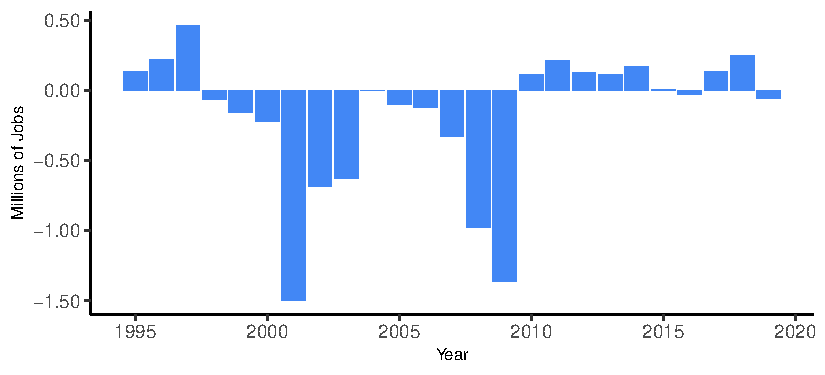
\includegraphics{Final-Draft_files/figure-latex/unnamed-chunk-3-1} \end{center}



\FloatBarrier
\begin{figurenotes}
Annual net change in manufacturing employment in the United States. 
\end{figurenotes}
\end{figure}
\FloatBarrier

\section{Data and Methods} 
\label{datamethods}

\subsection{Data} 
\label{datasec}

Following \cite{Baccini21}, our unit of analysis is the county. This
allows us to capture not only the direct effects of deindustrialization
on laid-off manufacturing workers, but also possible spillover effects
on the greater population within the county. The primary outcome
variable is the county's change in Democratic vote share between 2012
and 2016. We obtain data on election outocmes and various covariate
terms from the publically-available replication data provided by
\cite{Baccini21}.

We want to measure the causal relationship between deindustrialization
and the change in vote share. As a measure of deindustrialization, we
use the loss of manufacturing jobs as a share of the total
beginning-of-period employment in each county. Suppose at the beginning
of our period there were \(2000\) manufacturing workers in a county, and
\(8000\) non-manufacturing workers. At the end there are only \(1500\)
manufacturing workers. Using our measure of net change in manufacturing
employment, this is a loss of \(500/10000 = 5\%.\)

In this choice we diverge from \cite{Baccini21}, which uses \emph{gross}
manufacturing job losses. For example, if a county lost \(450\)
manufacturing jobs from 2012-2015 and also gained \(400\) manufacturing
jobs over the same period, this would be \(450\) \emph{gross} job
losses, but only \(50\) \emph{net} job losses. The \emph{gross} measure
captures several dynamics unrelated to deindustrialization - for
example, seasonal unemployment in a food-manufacturing region, or
workers moving between jobs. Thus we believe the \emph{net} job losses
over a period are the more accurate measure. Additionally, there is
precedent in the literature to use \emph{net} employment changes, as
\cite{Autor21} have done. Nevertheless, it can be argued that the
non-seasonal or non-structural components of gross job losses are a
useful covariate. For instance, basic notions of prospect theory suggest
that the loss of a job and subsequent regaining of another identical job
may still create substantial discontent. Constructing a better measure
of gross job losses is an area for further methodological and
substantive research.

Data on job gains and losses are obtained, using an API, from the Census
Bureau's Quarterly Workforce Indicators (\cite{QWI}), which contains
(among other things) information about employment by industry and
county. These statistics are further disaggregated by race and
ethnicity. The Census Bureau obtains this data from a combination of
sources, such as administrative tax data and the U.S. Census.

Basic descriptive statistics of job losses and other key covariates can
be seen in Table \ref{tab:descTable}. \FloatBarrier

\begin{table}[!h]

\caption{\label{tab:descTable}Manufacturing Job Changes 2004-2015}
\centering
\resizebox{\linewidth}{!}{
\begin{tabular}[t]{lrrrrr}
\toprule
  & Mean & Std Dev & 25th Pctile & Median & 75th Pctile\\
\midrule
Mfg Share of Emp & 0.20 & 0.15 & 0.09 & 0.17 & 0.29\\
Mfg Share of Emp (White) & 0.16 & 0.13 & 0.06 & 0.13 & 0.22\\
Mfg Share of Emp (Nonwhite) & 0.05 & 0.07 & 0.01 & 0.02 & 0.06\\
Change in Mfg Jobs/ Worker & 0.04 & 0.09 & -0.01 & 0.02 & 0.06\\
Change in Mfg Jobs/ Worker (W) & 0.03 & 0.07 & 0.00 & 0.02 & 0.06\\
\addlinespace
Change in Mfg Jobs/ Worker (NW) & 0.00 & 0.04 & -0.01 & 0.00 & 0.01\\
\bottomrule
\end{tabular}}
\end{table}
\FloatBarrier

\subsection{Methods} 
\label{methodssec}

We conduct two related tests of our hypothesis. Our first test involves
an instrumental-variable approach. A regression of change in Democratic
vote share on manufacturing job losses risks endogeneity, in case
counties with manufacturing job losses were otherwise predisposed to
turn towards Trump (a singular candidate, after all). To mitigate these
risks, \cite{Baccini21} use a Bartik instrument, which we adapt (see
\cite{Bartik91}). This instrument essentially uses the cross-county
distribution of manufacturing employment as a source of exogenous
variation.

\[
\begin{aligned}
b_{j,c} &=& \frac{\text{Manufacturing Employment}_{j,c} \text{ at } t_0}{\text{Total Employment}_c \text{ at }t_0}  \\
&&  * \frac{\text{National Manufacturing Job Change}_{j,c} }{\text{Total National Employment at }t_0} \\
\end{aligned}
\]

Using this instrument, we then conduct a two-stage regression. First we
estimate manufacturing job loss with the Bartik Instrument and a set of
county-level controls; then we use the estimated values of job losses to
predict Democratic vote share. In these regressions we control for
unemployment, the share of college-educated voters, and the share of
male voters. For some estimates, we also control for the white share of
the population and service layoffs. We also apply state fixed effects to
account for a wide variety of state-level changes from 2012-2016 (such
as voter suppression tactics). These controls are similar to those of
\cite{Baccini21}.

Our second approach involves attempting to balance the covariates of the
deindustrialization treatment. We use the same covariates as are used in
controls above, as well as manufacturing as share of the population and
total population. We apply the method of Covariate Balancing Propensity
Scores, as developed by \cite{Imai14}; this method generates weights to
reduce the correlation between covariates and treatment, while
addressing several of the issues with propensity score weights. Given
covariate-balancing weights, we then conduct a single-stage weighted
regression of change in Democratic vote share on manufacturing job loss,
using the same controls as above.

XXXXXXXXXXXXXXX BALANCE FIGURE??? XXXXXXXXXXXXXXXXXXXXXXXXXXX

\subsection{Results}

We find that counties experiencing deindustrialization from 2004-2015
are substantially more likely to vote for Trump. Further, we find that
this effect is largely attributable to whites. In other words, net white
manufacturing job losses decreased Democratic vote share, while net
non-white manufacturing job losses increased Democratic vote share. We
find the same effect when using covariate balancing, albeit of reduced
size.

The results can be found in Table \ref{regResult04}. The regression
coefficient in Model 4, for instance, means that a loss of \(10\) white
manufacturing jobs per \(100\) workers in a county (a relatively extreme
value) corresponds to a \(3.2\) percentage point loss in Democratic vote
share. \FloatBarrier

\begin{table}[!htbp] \centering 
  \caption{Effect of Manufacturing Job Loss from 2004 to 2015} 
  \label{regResult04} 
\begin{tabular}{@{\extracolsep{5pt}}lcccc} 
\\[-1.8ex]\hline 
\hline \\[-1.8ex] 
 & \multicolumn{4}{c}{\textit{Dependent variable:}} \\ 
\cline{2-5} 
\\[-1.8ex] & \multicolumn{4}{c}{Change in Dem. Share, 2016-2012} \\ 
\\[-1.8ex] & (1) & (2) & (3) & (4)\\ 
\hline \\[-1.8ex] 
 Manufacturing Layoffs & $-$0.34$^{**}$ & $-$0.38$^{**}$ &  &  \\ 
  & (0.14) & (0.17) &  &  \\ 
  & & & & \\ 
 White Manufacturing Layoffs &  &  & $-$0.23$^{***}$ & $-$0.32$^{***}$ \\ 
  &  &  & (0.08) & (0.10) \\ 
  & & & & \\ 
 Nonwhite Manufacturing Layoffs &  &  & 0.15$^{***}$ & 0.20$^{***}$ \\ 
  &  &  & (0.05) & (0.06) \\ 
  & & & & \\ 
\hline \\[-1.8ex] 
White Share/Svc Layoffs Control & No & Yes & No & Yes \\ 
Observations & 3,049 & 3,049 & 2,750 & 2,750 \\ 
Adjusted R$^{2}$ & 0.72 & 0.72 & 0.75 & 0.75 \\ 
\hline 
\hline \\[-1.8ex] 
\textit{Note:}  & \multicolumn{4}{r}{$^{*}$p$<$0.1; $^{**}$p$<$0.05; $^{***}$p$<$0.01} \\ 
\end{tabular} 
\end{table} 
\FloatBarrier

This coefficient is still somewhat difficult to interpret, and made
increasingly so by the winner-take-all system by which U.S. Electoral
College votes are allocated. As an alternative perspective, we examined
a range of counterfactual scenarios, in which counties manufacturing
experienced job losses between the 1st and 99th percentiles across all
counties.

For example, in the map below, we assume that all counties in the US
experienced a loss in white manufacturing employment equivalent to the
level experienced by a county at the 25th percentile. Here, that level
is equivalent to a 0 net loss in white manufacturing jobs between
2004-2015 per 100 workers in 2004 (a relatively low level of job
losses). Setting all counties' white manufacturing job losses to 0, we
use the point estimates of our regression coefficients from Model 3 in
Table \ref{regResult04} to estimate the counterfactual change in
Democratic vote share. We find that, had all counties experienced the
25th percentile level in manufacturing job losses, most states would
have leaned more Democratic in 2016, and that Michigan and Pennsylvania
would have flipped.

\FloatBarrier
\begin{figure} \label{counterfactual1}
\caption{Counterfactual Scenario: Change in Democratic Vote Share Assuming 25th Percentile of Manufacturing Job Losses}

\begin{center}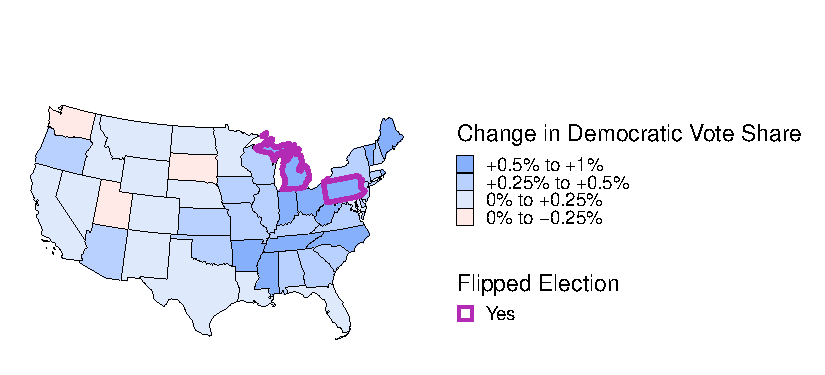
\includegraphics{Final-Draft_files/figure-latex/unnamed-chunk-6-1} \end{center}



\FloatBarrier
\end{figure}
\FloatBarrier

\FloatBarrier
\begin{figure} \label{counterfactual2}

\caption{Counterfactual Simulation Results: Democratic Electoral College Votes Assuming White Manufacturing Job Losses Between 1st and 99th Percentile }

\begin{center}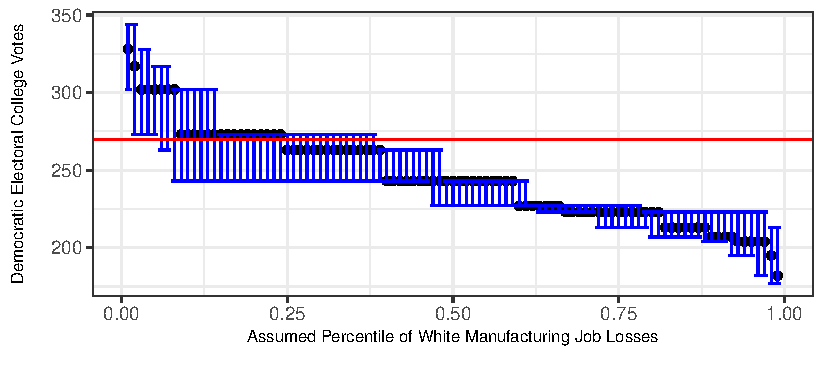
\includegraphics{Final-Draft_files/figure-latex/unnamed-chunk-7-1} \end{center}



\FloatBarrier
\end{figure}
\begin{figurenotes}
Figures show a 95% confidence interval for Democratic Electoral College Votes at Each Percentile of Manufacturing Job Losses.
\end{figurenotes}
\FloatBarrier

\FloatBarrier
\begin{figure} \label{counterfactual3}
\caption{Clinton Winning Freq}

\begin{center}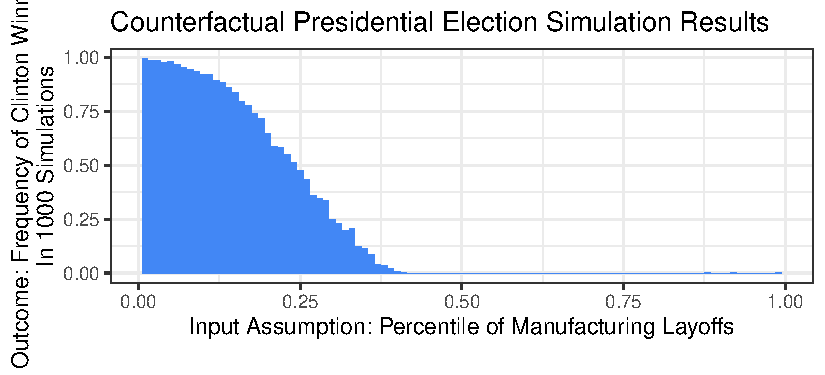
\includegraphics{Final-Draft_files/figure-latex/unnamed-chunk-8-1} \end{center}



\FloatBarrier
\end{figure}
\FloatBarrier
\subsubsection{Timing}

Restricting our analysis to only the 2012-2015 period, while continuing
to use the net job loss metric, produces an effect opposite to that of
\cite{Baccini21}. The loss of Democratic vote share seems to be
associated with a gain in manufacturing jobs, both in general and among
whites. We believe this time-restricted analysis suffers from an omitted
variable bias. As discussed above, the 2012-2015 period can be broadly
characterized as a slight rebound from the manufacturing job losses in
the 2008 financial crisis. The counties that experience job losses from
2004-2012 are more likely to have job gains in 2012-2015 (see
\ref{vShapePlot}). An apparent relationship between 2012-2015 job gains
and loss of Democratic vote share in fact represents 2004-2012 job
losses that may lead to both the later job gains and the loss of vote
share. These results can be seen in Table \ref{regResult12}.
\FloatBarrier

\begin{table}[!htbp] \centering 
  \caption{Effect of Manufacturing Job Loss from 2004 to 2015} 
  \label{regResult12} 
\begin{tabular}{@{\extracolsep{5pt}}lcccc} 
\\[-1.8ex]\hline 
\hline \\[-1.8ex] 
 & \multicolumn{4}{c}{\textit{Dependent variable:}} \\ 
\cline{2-5} 
\\[-1.8ex] & \multicolumn{4}{c}{Change in Dem. Share, 2016-2012} \\ 
\\[-1.8ex] & (1) & (2) & (3) & (4)\\ 
\hline \\[-1.8ex] 
 Manufacturing Layoffs & 0.43$^{**}$ & 0.37$^{**}$ &  &  \\ 
  & (0.17) & (0.17) &  &  \\ 
  & & & & \\ 
 White Manufacturing Layoffs &  &  & 6.50$^{***}$ & 2.33$^{***}$ \\ 
  &  &  & (2.20) & (0.76) \\ 
  & & & & \\ 
 Nonwhite Manufacturing Layoffs &  &  & $-$3.99$^{***}$ & $-$1.42$^{***}$ \\ 
  &  &  & (1.36) & (0.47) \\ 
  & & & & \\ 
\hline \\[-1.8ex] 
White Share/Svc Layoffs Control & No & Yes & No & Yes \\ 
Observations & 3,064 & 3,064 & 2,765 & 2,765 \\ 
Adjusted R$^{2}$ & 0.73 & 0.73 & 0.75 & 0.75 \\ 
\hline 
\hline \\[-1.8ex] 
\textit{Note:}  & \multicolumn{4}{r}{$^{*}$p$<$0.1; $^{**}$p$<$0.05; $^{***}$p$<$0.01} \\ 
\end{tabular} 
\end{table} 
\FloatBarrier

This result suggests an important temporal dimension to the political
effects of deindustrialization - job losses in 2004-2012 make their
effects felt in 2016. In some ways, this result is more plausible than
if the 2012-2015 job losses were a significant covariate of voting. The
effects of job loss may take some time to be felt, at both individual
and community levels (see \cite{Mckee09}, \cite{Foote19}). The
mechanisms of this relationship make a good topic for subsequent
research.

\subsection{Conclusion}

As much research has noted, the national and global implications of
American deindustrialization are only beginning to be felt - from the
2016 election to isolationism to the opioid epidemic. Previous analyses
have often focused on choosing between explanations grounded in racial
issues or political-economic evolutions (ex: \cite{Green19},
\cite{Reny19}). We are joining a growing body of scholars searching for
explanations at the intersection of the two. We believe that
deindustrialization is fundamentally connected to particular places, and
so the localized approach adopted by \cite{Baccini21} offers a great
deal of promise. Further research might explore further ways in which
geography has influenced the rightward turn in the U.S., for example
through the use of techniques of spatial econometrics or the careful use
of ethnography.

While our study is oriented towards history, deindustrialization is in
no way confined to the past. The trajectory of American manufacturing
employment is far from certain, with continued competition from abroad
and the perennial threat of automation. We believe the case of the U.S.
also offers insight that is applicable to the phenomenon of `premature
deindustrialization' in the developing world, and the concurrent growth
of populist parties in Hungary, Brazil, India and elsewhere
(\cite{Rodrik15}, \cite{Castillo16}).

\nocite{Stargazer}

\bibliographystyle{aea}
\bibliography{references}

\appendix

\section{Appendix}

\begin{figure} \label{vShapePlot}
\caption{V-Shaped Recovery in Manufacturing Job Losses}

\begin{center}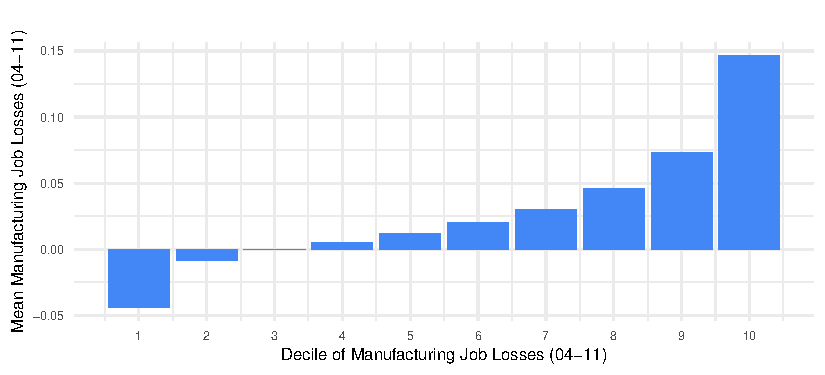
\includegraphics{Final-Draft_files/figure-latex/unnamed-chunk-10-1} \end{center}



\FloatBarrier
\begin{figurenotes}
"Stuff here"
\end{figurenotes}
\end{figure}

\begin{figure} \label{vShapePlot}
\caption{V-Shaped Recovery in Manufacturing Job Losses}

\begin{center}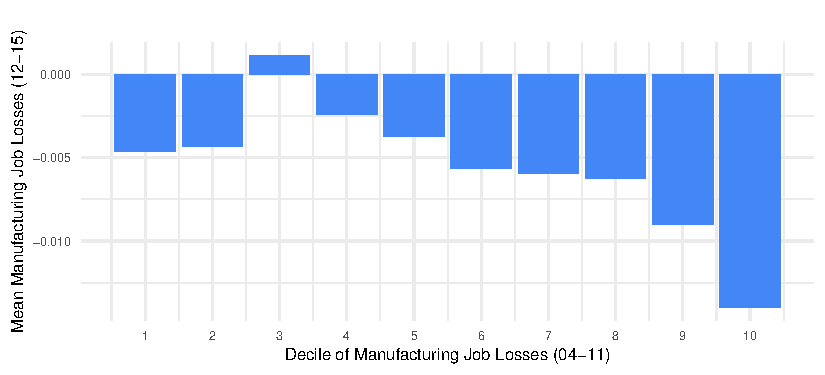
\includegraphics{Final-Draft_files/figure-latex/unnamed-chunk-11-1} \end{center}



\FloatBarrier

\begin{figurenotes}
"Stuff here"
\end{figurenotes}
\end{figure}

\end{document}

